\chapter{Sviluppi futuri}

\section{Possibile utilizzo di SADAM}

In una ricerca del 2018 Ballé introduce SpectralADAM (SADAM) \cite{balle2018efficient}, un'alternativa all’algoritmo ADAM \cite{kingma2014adam}, per l’addestramento di reti di compressione.\\
Se consideriamo una funzione di perdita $L$ che consiste in una somma di funzioni di una proiezione lineare dei vettori in input $x$ \ref{eq:SGDLoss}, dove $H$ è una matrice di filtri $h_{i}$. I filtri sono una parte dei parametri che devono essere ottimizzati in fase di addestramento, per ogni filtro la regola di aggiornamento del gradient descent \ref{eq:SGDUpdate} sottrae il gradiente della funzione di perdita moltiplicato per lo step size $\rho$.\\
\begin{equation}\label{eq:SGDLoss}
L = \sum_{x} l(x) \:\: \textrm{with} \:\: z = Hx
\end{equation}\\
\begin{equation}\label{eq:SGDUpdate}
\Delta h = - \rho \dfrac{\partial L}{\partial h} = - \rho \sum_{x} \dfrac{\partial l}{\partial z} x
\end{equation}\\
L’aggiornamento $\Delta H$ consiste in somme scalari di vettori $x$ proiettate sui filtri corrispondenti, quindi ereditano la maggior parte della struttura della covarianza dei dati in input. Di conseguenza se $x$ fa parte di un insieme di immagini naturali abbiamo che lo spettro della potenza è inversamente proporzionale a quello della frequenza \cite{field1987relations}, dunque lo step size per componenti a basse frequenze è molto più grande rispetto a componenti ad alte frequenze, questo può portare a problemi di convergenza e in casi rari di stabilità.\\
Un metodo per risolvere questo problema è l’uso di un algoritmo diverso, simile al gradient descent, l’algoritmo ADAM \cite{kingma2014adam}, la cui funzione di aggiornamento \ref{eq:adamUpdate} varia leggermente. Dove $m_{h}$ è una media costantemente aggiornata della derivata $\tfrac{\partial l}{\partial z}$ e $C_{h}$ è una matrice diagonale che rappresenta la stima della covarianza.\\
\begin{equation}\label{eq:adamUpdate}
\Delta h = - \rho C_{h}^{-\tfrac{1}{2}} m_{h}
\end{equation}\\
Essendo $C_{h}$ forzata ad essere diagonale non riesce a rappresentare adeguatamente la struttura della covarianza per immagini naturali.\\
Per risolvere questo problema Ballé propone una variante di questo algoritmo, SpectralADAM, dove invece di applicare l’algoritmo direttamente ad $h$, viene applicato alla sua Trasformata Discreta di Fourier con ingresso Reale (RDFT) riparametrizzando $h$ \ref{eq:sadamH}.\\
\begin{equation}\label{eq:sadamH}
H = F^{T} g \:\: \textrm{with} \:\: g = Fx
\end{equation}\\
Per ottimizzare $g$ usiamo la derivata \ref{eq:sadamGradient} ed applichiamo la regola di aggiornamento \ref{eq:adamUpdate}.\\
\begin{equation}\label{eq:sadamGradient}
\dfrac{\partial l}{\partial g} = F \dfrac{\partial L}{\partial h} = - \dfrac{\partial l}{\partial z} Fx
\end{equation}\\
Essendo \ref{eq:sadamH} lineare possiamo calcolare l’aggiornamento $h$ come descritto nell’equazione \ref{eq:sadamUpdate}, dove $m_{g}$ e $C_{g}$ sono delle medie costantemente aggiornate delle derivate \ref{eq:sadamGradient} \\
\begin{equation}\label{eq:sadamUpdate}
\Delta h = F^{T} (-\rho C_{g}^{-\tfrac{1}{2}} m_{g}) = - \rho F^{T} C_{g}^{-\tfrac{1}{2}} Fm_{h}
\end{equation}\\
La stima della covaranza $ F^{T} C_{g} F$ deve essere diagonale nel dominio della trasformata di Fourier, non più nel dominio dei coefficienti dei filtri, e fino a quando $x$ è invariante per permutazioni, come tutti i dati spazio temporali, la base $F$ è garantito dia una buona approssimazione degli autovettori della vera struttura della covarianza dell’input $x$.\\
Dai risultati sperimentali della ricerca di Ballé, SADAM stabilizza e velocizza il processo di addestramento delle reti, inoltre essendo Ballé un ricercatore per Google, aveva già implementato il codice per queste soluzioni alternative all’interno della popolare libreria Tensorflow \cite{tensorflow2015-whitepaper}.\\
Alla luce di questi risultati ottenuti da Ballé ci chiediamo come mai negli anni successivi questo metodo non sia stato utilizzato per addestrare le nuove reti, ma si sia preferito continuare ad usare ADAM, come possiamo vedere nei lavori di Cheng et al. \cite{cheng2020learned} e Wang et al. \cite{wang2022neural}. Riteniamo quindi sarebbe interessante addestrare nuovamente queste reti utilizzando SADAM e valutare la differenza di prestazioni.


\section{Utilizzi in dispositivi mobili con Slim CAE}

Durante la ricerca delle fonti per la stesura di questo documento ci siamo imbattuti in una ricerca molto interessante del 2021 da parte di Yang et al. \cite{yang2021slimmable}, dove propongono di utilizzare delle SlimCAE, in modo da poter ridurre la potenza di calcolo necessaria per la compressione senza rinunciare a troppa qualità, tutto questo per poter rendere questa tecnologia fruibile anche su dispositivi con ridotta potenza di calcolo, come gli smartphone o più in generale dei dispositivi mobili.\\
Per rendere gli autoencoder, la cui struttura è stata descritta nel capitolo 2, degli slimmable autoencoder è necessario rendere i vali livelli della rete slimmable. Un livello, per essere slimmable, deve realizzare un’operazione valida rimuovendo parte dei parametri di quel livello.\\
Consideriamo gli slimAE come composti da $K$ sotto autoencoders, ognuno caratterizzato da due parametri \ref{eq:slimAEParameters} ed ognuno con la sua funzione di perdita \ref{eq:slimAELoss}. Di conseguenza i parametri di tutta la rete sono contenuti in un vettore di $K$ coppie di parametri e la funzione di perdita altro non è che la somma pesata, con dei pesi $w^{k}$, delle $K$ funzioni di perdita.\\
\begin{equation}\label{eq:slimAEParameters}
\psi^{k} = (\theta^{(k)},\phi^{(k)}) \:\: \in \:\: {(\theta^{(1)},\phi^{(1)}),\,…\, , (\theta^{(K)},\phi^{(K)})}
\end{equation}\\
\begin{equation}\label{eq:slimAELoss}
L(\Psi, \chi) = \sum_{k} w^{k} L^{k} (\theta^{k}, \phi^{k}; \chi)
\end{equation}\\
Per ottenere invece delle slimCAE dobbiamo rendere tutte le operazioni nei CAE non parametriche, riducibili o rimpiazzabili senza perdere efficienza. Nella rete proposta da Yang et al. la quantizzazione non è parametrica, i livelli convoluzionali sono stati implementati per essere riducibili, per GDN e IGND \cite{balle2018efficient} ci sono varie alternative che possono essere intercambiate ed infine vengono utilizzati dei modelli per l’entropia scambiabili, in questo modo ogni sotto CAE ha i suoi parametri $\nu^{k}$.\\
Possiamo vedere uno schema di funzionamento di una slimCAE nell’immagine \ref{fig:smallCAE}, osserviamo come andando ad incrementare la dimensione della rete possiamo comprimere più dettagli, realizzando quindi una codifica progressiva.\\
Dai risultati sperimentali ottenuti dal team di Yang et al. \cite{yang2021slimmable}, la rete da loro proposta ottiene risultati al pari del modello proposto da Ballé et al. \cite{minnen2018joint}, nonostante le dimensioni ridotte della rete e i tempi di codifica ridotti.\\
Ci chiediamo quindi come mai questo modello non abbia guadagnato popolarità data la sua applicabilità in situazioni più vicine alla realtà e per quale motivo le nuove reti non cerchino di realizzare anche delle versioni riducibili per permettere a sempre più persone di usufruire di tale tecnologia.\\
\begin{figure}[!h]
    \centering
    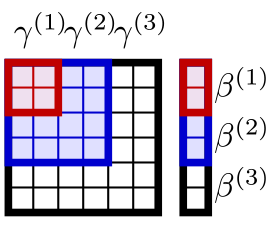
\includegraphics[width=0.4\textwidth]{Immagini/slimCAE.png}
    \caption{Diagramma funzionamento slimCAE, immagine presa dal documento \cite{yang2021slimmable}}
    \label{fig:smallCAE}
\end{figure}